\documentclass[twoside]{book}

% Packages required by doxygen
\usepackage{fixltx2e}
\usepackage{calc}
\usepackage{doxygen}
\usepackage[export]{adjustbox} % also loads graphicx
\usepackage{graphicx}
\usepackage[utf8]{inputenc}
\usepackage{makeidx}
\usepackage{multicol}
\usepackage{multirow}
\PassOptionsToPackage{warn}{textcomp}
\usepackage{textcomp}
\usepackage[nointegrals]{wasysym}
\usepackage[table]{xcolor}

% Font selection
\usepackage[T1]{fontenc}
\usepackage[scaled=.90]{helvet}
\usepackage{courier}
\usepackage{amssymb}
\usepackage{sectsty}
\renewcommand{\familydefault}{\sfdefault}
\allsectionsfont{%
  \fontseries{bc}\selectfont%
  \color{darkgray}%
}
\renewcommand{\DoxyLabelFont}{%
  \fontseries{bc}\selectfont%
  \color{darkgray}%
}
\newcommand{\+}{\discretionary{\mbox{\scriptsize$\hookleftarrow$}}{}{}}

% Page & text layout
\usepackage{geometry}
\geometry{%
  a4paper,%
  top=2.5cm,%
  bottom=2.5cm,%
  left=2.5cm,%
  right=2.5cm%
}
\tolerance=750
\hfuzz=15pt
\hbadness=750
\setlength{\emergencystretch}{15pt}
\setlength{\parindent}{0cm}
\setlength{\parskip}{0.2cm}
\makeatletter
\renewcommand{\paragraph}{%
  \@startsection{paragraph}{4}{0ex}{-1.0ex}{1.0ex}{%
    \normalfont\normalsize\bfseries\SS@parafont%
  }%
}
\renewcommand{\subparagraph}{%
  \@startsection{subparagraph}{5}{0ex}{-1.0ex}{1.0ex}{%
    \normalfont\normalsize\bfseries\SS@subparafont%
  }%
}
\makeatother

% Headers & footers
\usepackage{fancyhdr}
\pagestyle{fancyplain}
\fancyhead[LE]{\fancyplain{}{\bfseries\thepage}}
\fancyhead[CE]{\fancyplain{}{}}
\fancyhead[RE]{\fancyplain{}{\bfseries\leftmark}}
\fancyhead[LO]{\fancyplain{}{\bfseries\rightmark}}
\fancyhead[CO]{\fancyplain{}{}}
\fancyhead[RO]{\fancyplain{}{\bfseries\thepage}}
\fancyfoot[LE]{\fancyplain{}{}}
\fancyfoot[CE]{\fancyplain{}{}}
\fancyfoot[RE]{\fancyplain{}{\bfseries\scriptsize Generated on Wed May 6 2015 16\+:56\+:21 for M\+D\+L\+Participant by Doxygen }}
\fancyfoot[LO]{\fancyplain{}{\bfseries\scriptsize Generated on Wed May 6 2015 16\+:56\+:21 for M\+D\+L\+Participant by Doxygen }}
\fancyfoot[CO]{\fancyplain{}{}}
\fancyfoot[RO]{\fancyplain{}{}}
\renewcommand{\footrulewidth}{0.4pt}
\renewcommand{\chaptermark}[1]{%
  \markboth{#1}{}%
}
\renewcommand{\sectionmark}[1]{%
  \markright{\thesection\ #1}%
}

% Indices & bibliography
\usepackage{natbib}
\usepackage[titles]{tocloft}
\setcounter{tocdepth}{3}
\setcounter{secnumdepth}{5}
\makeindex

% Hyperlinks (required, but should be loaded last)
\usepackage{ifpdf}
\ifpdf
  \usepackage[pdftex,pagebackref=true]{hyperref}
\else
  \usepackage[ps2pdf,pagebackref=true]{hyperref}
\fi
\hypersetup{%
  colorlinks=true,%
  linkcolor=blue,%
  citecolor=blue,%
  unicode%
}

% Custom commands
\newcommand{\clearemptydoublepage}{%
  \newpage{\pagestyle{empty}\cleardoublepage}%
}


%===== C O N T E N T S =====

\begin{document}

% Titlepage & ToC
\hypersetup{pageanchor=false,
             bookmarks=true,
             bookmarksnumbered=true,
             pdfencoding=unicode
            }
\pagenumbering{roman}
\begin{titlepage}
\vspace*{7cm}
\begin{center}%
{\Large M\+D\+L\+Participant }\\
\vspace*{1cm}
{\large Generated by Doxygen 1.8.9.1}\\
\vspace*{0.5cm}
{\small Wed May 6 2015 16:56:21}\\
\end{center}
\end{titlepage}
\clearemptydoublepage
\tableofcontents
\clearemptydoublepage
\pagenumbering{arabic}
\hypersetup{pageanchor=true}

%--- Begin generated contents ---
\chapter{Namespace Index}
\section{Packages}
Here are the packages with brief descriptions (if available)\+:\begin{DoxyCompactList}
\item\contentsline{section}{\hyperlink{namespace_m_d_l_participants}{M\+D\+L\+Participants} }{\pageref{namespace_m_d_l_participants}}{}
\end{DoxyCompactList}

\chapter{Hierarchical Index}
\section{Class Hierarchy}
This inheritance list is sorted roughly, but not completely, alphabetically\+:\begin{DoxyCompactList}
\item \contentsline{section}{M\+D\+L\+Participants.\+Bdd}{\pageref{class_m_d_l_participants_1_1_bdd}}{}
\item Form\begin{DoxyCompactList}
\item \contentsline{section}{M\+D\+L\+Participants.\+Frm\+Login}{\pageref{class_m_d_l_participants_1_1_frm_login}}{}
\item \contentsline{section}{M\+D\+L\+Participants.\+Frm\+Principale}{\pageref{class_m_d_l_participants_1_1_frm_principale}}{}
\end{DoxyCompactList}
\end{DoxyCompactList}

\chapter{Class Index}
\section{Class List}
Here are the classes, structs, unions and interfaces with brief descriptions\+:\begin{DoxyCompactList}
\item\contentsline{section}{\hyperlink{class_m_d_l_participants_1_1_bdd}{M\+D\+L\+Participants.\+Bdd} }{\pageref{class_m_d_l_participants_1_1_bdd}}{}
\item\contentsline{section}{\hyperlink{class_m_d_l_participants_1_1_frm_login}{M\+D\+L\+Participants.\+Frm\+Login} }{\pageref{class_m_d_l_participants_1_1_frm_login}}{}
\item\contentsline{section}{\hyperlink{class_m_d_l_participants_1_1_frm_principale}{M\+D\+L\+Participants.\+Frm\+Principale} }{\pageref{class_m_d_l_participants_1_1_frm_principale}}{}
\end{DoxyCompactList}

\chapter{Namespace Documentation}
\hypertarget{namespace_m_d_l_participants}{}\section{Package M\+D\+L\+Participants}
\label{namespace_m_d_l_participants}\index{M\+D\+L\+Participants@{M\+D\+L\+Participants}}
\subsection*{Classes}
\begin{DoxyCompactItemize}
\item 
class \hyperlink{class_m_d_l_participants_1_1_bdd}{Bdd}
\item 
class \hyperlink{class_m_d_l_participants_1_1_frm_login}{Frm\+Login}
\item 
class \hyperlink{class_m_d_l_participants_1_1_frm_principale}{Frm\+Principale}
\item 
class {\bfseries Program}
\end{DoxyCompactItemize}

\chapter{Class Documentation}
\hypertarget{class_m_d_l_participants_1_1_bdd}{}\section{M\+D\+L\+Participants.\+Bdd Class Reference}
\label{class_m_d_l_participants_1_1_bdd}\index{M\+D\+L\+Participants.\+Bdd@{M\+D\+L\+Participants.\+Bdd}}
\subsection*{Public Member Functions}
\begin{DoxyCompactItemize}
\item 
\hyperlink{class_m_d_l_participants_1_1_bdd_a0b1573b8583b8a36d8b9badd7d4fea75}{Bdd} (String Un\+Login, String Un\+Pwd)
\begin{DoxyCompactList}\small\item\em constructeur de la connexion \end{DoxyCompactList}\item 
Data\+Table \hyperlink{class_m_d_l_participants_1_1_bdd_abd7da8d1db22121522c19981fadb8a49}{Obtenir\+Donnes\+Oracle} (String Une\+Table\+Ou\+Vue)
\begin{DoxyCompactList}\small\item\em permet de récupérer le contenu d\textquotesingle{}une table ou d\textquotesingle{}une vue. \end{DoxyCompactList}\item 
\hypertarget{class_m_d_l_participants_1_1_bdd_a0f7bc6534737252b49e36318ba2005b2}{}void {\bfseries Ajout\+Date\+Heure\+Arrivee\+Participant} (Int16 p\+Id\+Participant, Date\+Time p\+Date\+Heure\+Arrivee, String p\+Cle\+Wifi)\label{class_m_d_l_participants_1_1_bdd_a0f7bc6534737252b49e36318ba2005b2}

\end{DoxyCompactItemize}
\subsection*{Static Public Member Functions}
\begin{DoxyCompactItemize}
\item 
static void \hyperlink{class_m_d_l_participants_1_1_bdd_a2b5d8e9ad5405fdf4522e1d2e82d13f1}{Remplir\+Combo\+Box} (\hyperlink{class_m_d_l_participants_1_1_bdd}{Bdd} Une\+Connexion, Combo\+Box Une\+Combo, String Une\+Source)
\begin{DoxyCompactList}\small\item\em méthode permettant de remplir une combobox à partir d\textquotesingle{}une source de données \end{DoxyCompactList}\end{DoxyCompactItemize}


\subsection{Constructor \& Destructor Documentation}
\hypertarget{class_m_d_l_participants_1_1_bdd_a0b1573b8583b8a36d8b9badd7d4fea75}{}\index{M\+D\+L\+Participants\+::\+Bdd@{M\+D\+L\+Participants\+::\+Bdd}!Bdd@{Bdd}}
\index{Bdd@{Bdd}!M\+D\+L\+Participants\+::\+Bdd@{M\+D\+L\+Participants\+::\+Bdd}}
\subsubsection[{Bdd}]{\setlength{\rightskip}{0pt plus 5cm}M\+D\+L\+Participants.\+Bdd.\+Bdd (
\begin{DoxyParamCaption}
\item[{String}]{Un\+Login, }
\item[{String}]{Un\+Pwd}
\end{DoxyParamCaption}
)}\label{class_m_d_l_participants_1_1_bdd_a0b1573b8583b8a36d8b9badd7d4fea75}


constructeur de la connexion 


\begin{DoxyParams}{Parameters}
{\em Un\+Login} & login utilisateur\\
\hline
{\em Un\+Pwd} & mot de passe utilisateur\\
\hline
\end{DoxyParams}
on commence par récupérer dans Cn\+String les informations contenues dans le fichier app.\+config pour la connection\+String de nom Str\+Conn\+Mdl 

on va remplacer dans la chaine de connexion les paramètres par le login et le pwd saisis dans les zones de texte. Pour ça on va utiliser la méthode Format de la classe String. /// 

\subsection{Member Function Documentation}
\hypertarget{class_m_d_l_participants_1_1_bdd_abd7da8d1db22121522c19981fadb8a49}{}\index{M\+D\+L\+Participants\+::\+Bdd@{M\+D\+L\+Participants\+::\+Bdd}!Obtenir\+Donnes\+Oracle@{Obtenir\+Donnes\+Oracle}}
\index{Obtenir\+Donnes\+Oracle@{Obtenir\+Donnes\+Oracle}!M\+D\+L\+Participants\+::\+Bdd@{M\+D\+L\+Participants\+::\+Bdd}}
\subsubsection[{Obtenir\+Donnes\+Oracle}]{\setlength{\rightskip}{0pt plus 5cm}Data\+Table M\+D\+L\+Participants.\+Bdd.\+Obtenir\+Donnes\+Oracle (
\begin{DoxyParamCaption}
\item[{String}]{Une\+Table\+Ou\+Vue}
\end{DoxyParamCaption}
)}\label{class_m_d_l_participants_1_1_bdd_abd7da8d1db22121522c19981fadb8a49}


permet de récupérer le contenu d\textquotesingle{}une table ou d\textquotesingle{}une vue. 


\begin{DoxyParams}{Parameters}
{\em Une\+Table\+Ou\+Vue} & nom de la table ou la vue dont on veut récupérer le contenu\\
\hline
\end{DoxyParams}
\begin{DoxyReturn}{Returns}
un objet de type datatable contenant les données récupérées
\end{DoxyReturn}
\hypertarget{class_m_d_l_participants_1_1_bdd_a2b5d8e9ad5405fdf4522e1d2e82d13f1}{}\index{M\+D\+L\+Participants\+::\+Bdd@{M\+D\+L\+Participants\+::\+Bdd}!Remplir\+Combo\+Box@{Remplir\+Combo\+Box}}
\index{Remplir\+Combo\+Box@{Remplir\+Combo\+Box}!M\+D\+L\+Participants\+::\+Bdd@{M\+D\+L\+Participants\+::\+Bdd}}
\subsubsection[{Remplir\+Combo\+Box}]{\setlength{\rightskip}{0pt plus 5cm}static void M\+D\+L\+Participants.\+Bdd.\+Remplir\+Combo\+Box (
\begin{DoxyParamCaption}
\item[{{\bf Bdd}}]{Une\+Connexion, }
\item[{Combo\+Box}]{Une\+Combo, }
\item[{String}]{Une\+Source}
\end{DoxyParamCaption}
)\hspace{0.3cm}{\ttfamily [static]}}\label{class_m_d_l_participants_1_1_bdd_a2b5d8e9ad5405fdf4522e1d2e82d13f1}


méthode permettant de remplir une combobox à partir d\textquotesingle{}une source de données 


\begin{DoxyParams}{Parameters}
{\em Une\+Connexion} & L\textquotesingle{}objet connexion à utiliser pour la connexion à la B\+D\\
\hline
{\em Une\+Combo} & La combobox que l\textquotesingle{}on doit remplir\\
\hline
{\em Une\+Source} & Le nom de la source de données qui va fournir les données. Il s\textquotesingle{}agit en fait d\textquotesingle{}une vue de type V\+X\+X\+X\+X\+On ou X\+X\+X\+X représente le nom de la tabl à partir de laquelle la vue est créée. n représente un numéro de séquence\\
\hline
\end{DoxyParams}


The documentation for this class was generated from the following file\+:\begin{DoxyCompactItemize}
\item 
M\+D\+L\+Participants/\+M\+D\+L\+Participants/Bdd.\+cs\end{DoxyCompactItemize}

\hypertarget{class_m_d_l_participants_1_1_frm_login}{}\section{M\+D\+L\+Participants.\+Frm\+Login Class Reference}
\label{class_m_d_l_participants_1_1_frm_login}\index{M\+D\+L\+Participants.\+Frm\+Login@{M\+D\+L\+Participants.\+Frm\+Login}}
Inheritance diagram for M\+D\+L\+Participants.\+Frm\+Login\+:\begin{figure}[H]
\begin{center}
\leavevmode
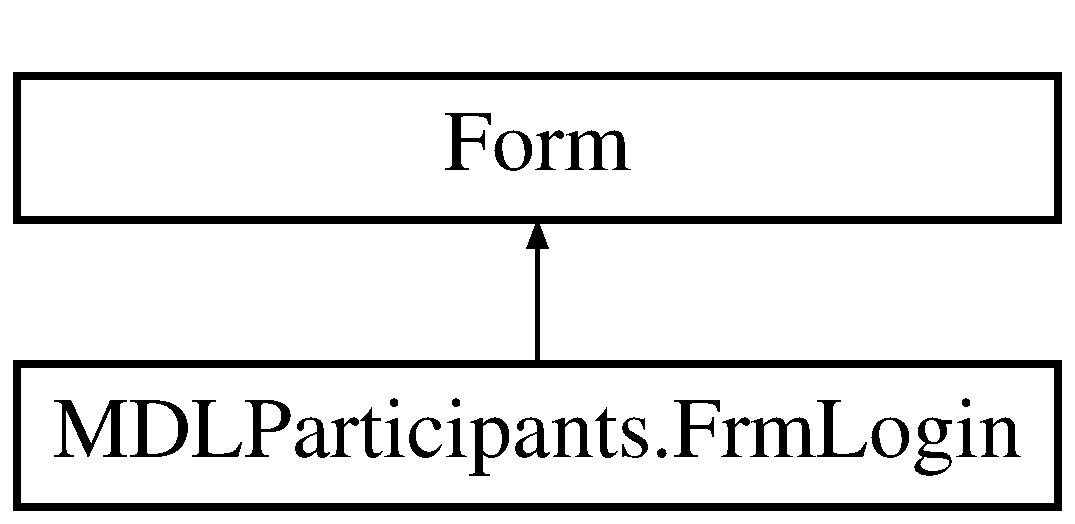
\includegraphics[height=2.000000cm]{class_m_d_l_participants_1_1_frm_login}
\end{center}
\end{figure}
\subsection*{Protected Member Functions}
\begin{DoxyCompactItemize}
\item 
override void \hyperlink{class_m_d_l_participants_1_1_frm_login_a29948d19b765c502fb40e9c531bb4b70}{Dispose} (bool disposing)
\begin{DoxyCompactList}\small\item\em Nettoyage des ressources utilisées. \end{DoxyCompactList}\end{DoxyCompactItemize}


\subsection{Member Function Documentation}
\hypertarget{class_m_d_l_participants_1_1_frm_login_a29948d19b765c502fb40e9c531bb4b70}{}\index{M\+D\+L\+Participants\+::\+Frm\+Login@{M\+D\+L\+Participants\+::\+Frm\+Login}!Dispose@{Dispose}}
\index{Dispose@{Dispose}!M\+D\+L\+Participants\+::\+Frm\+Login@{M\+D\+L\+Participants\+::\+Frm\+Login}}
\subsubsection[{Dispose}]{\setlength{\rightskip}{0pt plus 5cm}override void M\+D\+L\+Participants.\+Frm\+Login.\+Dispose (
\begin{DoxyParamCaption}
\item[{bool}]{disposing}
\end{DoxyParamCaption}
)\hspace{0.3cm}{\ttfamily [protected]}}\label{class_m_d_l_participants_1_1_frm_login_a29948d19b765c502fb40e9c531bb4b70}


Nettoyage des ressources utilisées. 


\begin{DoxyParams}{Parameters}
{\em disposing} & true si les ressources managées doivent être supprimées ; sinon, false.\\
\hline
\end{DoxyParams}


The documentation for this class was generated from the following files\+:\begin{DoxyCompactItemize}
\item 
M\+D\+L\+Participants/\+M\+D\+L\+Participants/Frm\+Login.\+cs\item 
M\+D\+L\+Participants/\+M\+D\+L\+Participants/Frm\+Login.\+Designer.\+cs\end{DoxyCompactItemize}

\hypertarget{class_m_d_l_participants_1_1_frm_principale}{}\section{M\+D\+L\+Participants.\+Frm\+Principale Class Reference}
\label{class_m_d_l_participants_1_1_frm_principale}\index{M\+D\+L\+Participants.\+Frm\+Principale@{M\+D\+L\+Participants.\+Frm\+Principale}}
Inheritance diagram for M\+D\+L\+Participants.\+Frm\+Principale\+:\begin{figure}[H]
\begin{center}
\leavevmode
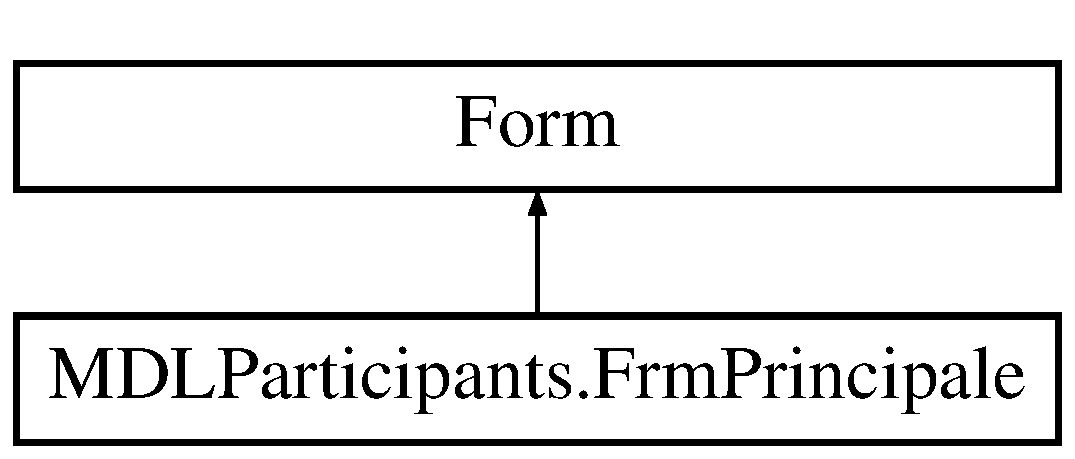
\includegraphics[height=2.000000cm]{class_m_d_l_participants_1_1_frm_principale}
\end{center}
\end{figure}
\subsection*{Public Member Functions}
\begin{DoxyCompactItemize}
\item 
\hypertarget{class_m_d_l_participants_1_1_frm_principale_a7437d2d5b3d27175d25d6a1025b5faf4}{}Date\+Time {\bfseries Get\+Date\+Fin\+Vacation} ()\label{class_m_d_l_participants_1_1_frm_principale_a7437d2d5b3d27175d25d6a1025b5faf4}

\item 
\hypertarget{class_m_d_l_participants_1_1_frm_principale_a76a5ff04d2e198edd649a23311b7db96}{}void {\bfseries show\+Image} (Image image)\label{class_m_d_l_participants_1_1_frm_principale_a76a5ff04d2e198edd649a23311b7db96}

\end{DoxyCompactItemize}
\subsection*{Protected Member Functions}
\begin{DoxyCompactItemize}
\item 
override void \hyperlink{class_m_d_l_participants_1_1_frm_principale_a755d6a66f41b95207a389f3991cfd6ad}{Dispose} (bool disposing)
\begin{DoxyCompactList}\small\item\em Clean up any resources being used. \end{DoxyCompactList}\end{DoxyCompactItemize}


\subsection{Member Function Documentation}
\hypertarget{class_m_d_l_participants_1_1_frm_principale_a755d6a66f41b95207a389f3991cfd6ad}{}\index{M\+D\+L\+Participants\+::\+Frm\+Principale@{M\+D\+L\+Participants\+::\+Frm\+Principale}!Dispose@{Dispose}}
\index{Dispose@{Dispose}!M\+D\+L\+Participants\+::\+Frm\+Principale@{M\+D\+L\+Participants\+::\+Frm\+Principale}}
\subsubsection[{Dispose}]{\setlength{\rightskip}{0pt plus 5cm}override void M\+D\+L\+Participants.\+Frm\+Principale.\+Dispose (
\begin{DoxyParamCaption}
\item[{bool}]{disposing}
\end{DoxyParamCaption}
)\hspace{0.3cm}{\ttfamily [protected]}}\label{class_m_d_l_participants_1_1_frm_principale_a755d6a66f41b95207a389f3991cfd6ad}


Clean up any resources being used. 


\begin{DoxyParams}{Parameters}
{\em disposing} & true if managed resources should be disposed; otherwise, false.\\
\hline
\end{DoxyParams}


The documentation for this class was generated from the following files\+:\begin{DoxyCompactItemize}
\item 
M\+D\+L\+Participants/\+M\+D\+L\+Participants/Frm\+Principale.\+cs\item 
M\+D\+L\+Participants/\+M\+D\+L\+Participants/Frm\+Principale.\+Designer.\+cs\end{DoxyCompactItemize}

%--- End generated contents ---

% Index
\backmatter
\newpage
\phantomsection
\clearemptydoublepage
\addcontentsline{toc}{chapter}{Index}
\printindex

\end{document}
